\subsection{Kn U claw}
La familia consiste en un grafo Kn y un grafo claw o estrella formado por un nodo y m nodos adyacentes, 
unidos de forma disjunta, que es luego complementado.
\begin{figure}[H]
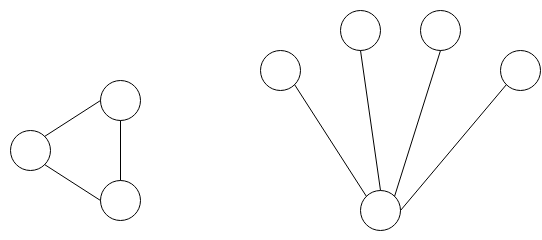
\includegraphics[width=80mm]{K3UC4.png}
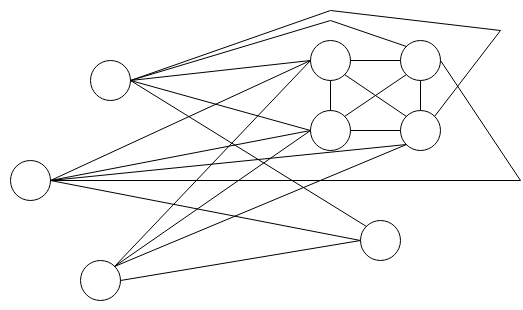
\includegraphics[width=80mm]{K3UC4Complemento.png}
\caption{La figura de la izquierda corresponde a K3 U claw 4, la figura derecha K3 U claw 4 complemento}
\label{overflow}
\end{figure}

\subsection{Grafo Completo K_n}
Un grafo completo es un grafo simple donde cada par de vértices está conectado por una arista.
Un grafo completo de n vértices tiene n(n-1)/2 aristas.
Es un grafo regular con todos sus vértices de grado n-1.

\begin{figure}[H]
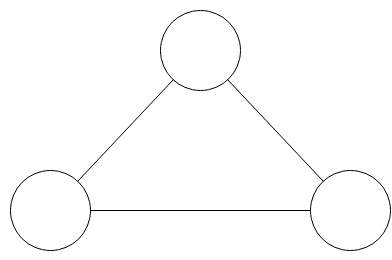
\includegraphics[width=80mm]{K3.png}
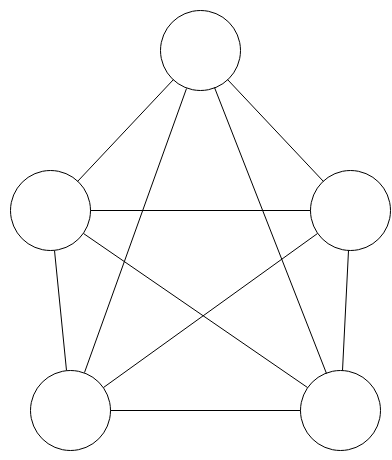
\includegraphics[width=80mm]{K5.png}
\caption{La figura de la izquierda corresponde a un grafo K_3 y la figura derecha a un grafo K_5}
\label{overflow}
\end{figure}